% Prepared by Calvin Kent
%
% Assignment Template v19.02
%
%%% 20xx0x/MATHxxx/Crowdmark/Ax
%
\documentclass[12pt]{article} %
\usepackage{CKpreamble}
\usepackage{CKassignment}
\usepackage{tkz-euclide}
\usepackage{physunits}
\usepackage{physics}
\usepackage{lmodern}
\usepackage{microtype}
\usepackage{upgreek}
\usepackage[misc]{ifsym}
\usepackage{graphicx}
\graphicspath{ {/home/user/Pictures/} }

%%% Maths and science packages

\usepackage{amsmath,amsthm,amssymb}
\usepackage{pgfplots}
	\usetikzlibrary{
		calc,
		patterns,
		positioning
	}
	\pgfplotsset{
		compat=1.16,
		samples=200,
		clip=false,
		my axis style/.style={
			axis x line=middle,
			axis y line=middle,
			legend pos=outer north east,
			axis line style={
				->,
			},
			legend style={
				font=\footnotesize
			},
			label style={
				font=\footnotesize
			},
			tick label style={
				font=\footnotesize
			},
			xlabel style={
				at={
					(ticklabel* cs:1)
				},
				anchor=west,
				font=\footnotesize,
			},
			ylabel style={
				at={
					(ticklabel* cs:1)
				},
				anchor=west,
				font=\footnotesize,
			},
			xlabel= $t$,
			ylabel=$\vec d (\m \tx{[East]})$
		},
	}
	\tikzset{
		>=stealth
	}

%%% Tables and figures packages

\usepackage{float}
\usepackage{caption}
	\captionsetup{
		format=plain,
		labelfont=bf,
		font=small,
		justification=centering
	}
	
%%% Numbers and sets

\newcommand{\E}{\mathrm{e}}

\newcommand{\tx}[1]{\text{#1}}

\begin{document}
    \pagenumbering{arabic}
    % Start of class settings ...
    \renewcommand*{\coursecode}{Physics REVIEW} % renew course code
    \renewcommand*{\assgnnumber}{1} % renew assignment number
    \renewcommand*{\submdate}{August 26, 2021} % renew the date
    \renewcommand*{\studentfname}{Abdullah} % Student first name
    \renewcommand*{\studentlname}{Zubair} % Student last name
    %\renewcommand*{\studentnum}{SNumber} % Student number

    \renewcommand\qedsymbol{$\blacksquare$}
    \setfigpath
    % End of class settings 
    \pagestyle{crowdmark}
    \newgeometry{left=18mm, right=18mm, top=22mm, bottom=22mm} % page is set to default values
    \fancyhfoffset[L,O]{0pt} % header orientation fixed
    % End of class settings
    %%% Note to user:
    % CTRL + F <CHANGE ME:> (without the angular brackets) in CKpreamble to specify graphics paths accordingly.
    % The command \circled[]{} accepts one optional and one mandatory argument.
    % Optional argument is for the size of the circle and mandatory argument is for its contents.
    % \circled{A} produces circled A, with size drawn for letter A. \circled[TT]{A} produces circled A with size drawn for TT.
    % https://github.com/CalvinKent/My-LaTeX
    %%%
    % Crowdmark assignment start
\begin{qstn}[1]
Answer the followiing True / False questions \textbf{(Assume [North],[East] is positive)}
\begin{enumerate}
\item I throw a rock $d = 100 \m$ in the air and it returns to my hand in $\Delta t = 20 \s$
	\begin{enumerate}[label = (\alph*)]
		\item The average speed of the ball was $v_{av} = 5 \m / \s$. (T / F) : \textcolor{blue}{F}
		\item The average velocity of the ball over $\Delta t = 20 \s$ was $\vec v_{av} = +5 \m / \s$[North]. (T / F) : \textcolor{blue}{F}
	\end{enumerate}
\item Suppose a rubber bullet travels at an average speed of $v_{av} = 600 \km / \s$ and an average velocity of $v_{av} = +600 \km / \s$.
	\begin{enumerate}[label = (\alph*)]
		\item The distance it can cover in $\Delta t = 4 \s$ is $d = 2.4 \times 10^6 \m$. (T / F) : \textcolor{blue}{F}
		\item Suppose the reference point is $(0,0)$. If the gun is placed at $\vec d_i = +20\m$ and then fired, then after $\Delta t = 2\s$, $\vec d_f = +1.2 \times 10^3\m$. (T / F)
	\end{enumerate}
\item Suppose that the equation of motion for a rocket was $x = -4t - 6$. Then,
	\begin{enumerate}[label = (\alph*)]
		\item The rocket experienced uniform motion. (T / F)
		\item The rocket experienced an average velocity of $\vec v_{av} = -10 \m / \s$. (T / F)
		\item The rocket was initially [West] relative to the reference point. (T / F)
	\end{enumerate}
\item Suppose that a frisbee has an average speed of $v_{av}$ and that it takes $\Delta t$ seconds to reach the end of the room. 
	\begin{enumerate}[label = (\alph*)]
		\item Doubling the average speed of the frisbee will triple the distance it can travel. (T / F)
		\item If I want the frisbee to reach the end of the room in $\frac{\Delta t}{3}$ seconds then I must triple the average speed. (T / F)
	\end{enumerate}
\item Consider the Position V. Time graph for a body in motion below
\begin{figure}[h]
	\begin{center}
	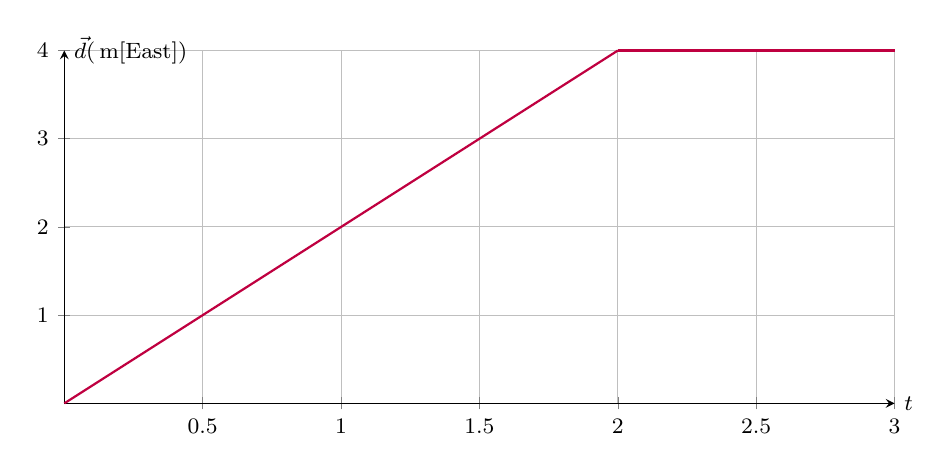
\begin{tikzpicture}
	\begin{axis}[
		my axis style,
		width=\textwidth,
		height=.5\textwidth,
		grid
	]
	
	\addplot[
		domain=0:2,
		thick,
		purple,
		-
	]
	{2*x};

	\addplot[
		domain=2:3,
		thick,
		purple,
		-
	]
	{4};
	
	\fill[
		black
	];
	
	\end{axis}
	\end{tikzpicture}
	\end{center}
\end{figure}
	\begin{enumerate}[label = (\alph*)]
		\item The body had an average velocity of $\vec v_{av} = +2 \m / \s$ over the time interval $[0,2]$. (T / F)
		\item The body experienced uniform motion over the entire trip. (T / F)
		\item The body continued to move at a non-zero velocity in the positive direction after $t = 2\s$. (T / F)
	\end{enumerate}


\item On an island there are three points $A,B,C$ that lie on a straight line. There is no information of $\vec d_{AB}$, I would like to obtain this vector. I can obtain this vector if there exists information of,
	\begin{enumerate}[label = (\alph*)]
		\item $\vec d_{AC}$, $\vec d_{BC}$. (T / F)
		\item $\vec d_{CA}$, $\vec d_{CB}$. (T / F)
		\item $\vec d_{AC}$, $\vec d_{CB}$. (T / F)
		\item $\vec d_{BC}$, $\vec d_{CA}$. (T / F)
		\item The average speed and the time elapsed from $A$, $B$. (T / F) 
	\end{enumerate}
 


\end{enumerate}


\end{qstn}



\begin{qstn}[2] % qnumber, qname, qpoints
	Convert the following quantities to $\m / \s$
	\begin{enumerate}[label = (\alph*)]
		\item $120 \mi / \h$
		\vspace*{4cm}

		\item $400 \km / \h$
		\vspace*{4cm}
		
		\item $368 \m / \min$
		\vspace*{4cm}

		\item $678 \inch / \min$
		\vspace*{4cm}

	\end{enumerate}

\end{qstn}


\begin{qstn}[3]
	Compute the \textbf{displacement} (or \emph{net} displacement) given the position vectors. Assume that the reference point is $(0,0)$ for \emph{all} vectors.
    \begin{enumerate}[label=(\alph*)]
        \item $\vec d_1 = 623 \tx{\m}[\tx{East}]$, $\vec d_2 = 412 \tx{\m}[\tx{West}]$

        \begin{soln}
            Lets make [East] positive,
            $$\Delta \vec d = \vec d_f - \vec d_i = -412 - 623 = -1135$$

        \end{soln}




        \item $\vec d_1 = +123\km$, $\vec d_2 = -81\km$, $\vec d_3 = -121\km$, $\vec d_4 = +610\km$, $\vec d_5 = +42\km$, $\vec d_6 = -742\m$.

        \begin{soln}
            $$\Delta \vec d = \vec d_f - \vec d_i = -742 - (+123) = -865$$

        \end{soln}



        \item $\vec d_i = 3\tx{\m}[\tx{East}]$, $\vec d_f = 4\tx{\m}[\tx{South}]$

        \begin{soln}
            $$\Delta \vec d = \vec d_f - \vec d_i =  $$

        \end{soln}



    \end{enumerate}

\end{qstn}


\begin{qstn}[4]
	Determine the sum/difference of the following vectors \textbf{\emph{geometrically}}. Use the $x-$dimensional coordinate system.
	\begin{enumerate}[label=(\alph*)]
		\item $\vec A = +3$, $\vec B = -6$ $$\vec A + \vec B$$
		\vspace*{7cm}
		\item $\vec A = +4$, $\vec B = +8$, $\vec C = -20$, $\vec D = -12$   $$\vec A + \vec B - (\vec C - \vec D)$$
		\newpage
		\item $\vec A = +2$, $\vec B = +18$, $\vec C = -12$, $\vec D = -8$, $\vec E = +7$  $$-\vec A  + \vec B + \vec C - \vec D + \vec E$$
		\vspace*{7cm}
	\end{enumerate}

\end{qstn}

\begin{qstn}[5]
Suppose that vehicle has an average velocity of $\vec v_{av} = -3 \m / \s$. Suppose that he is initially at a position $\vec d_i = +5 \m$ relative to the reference point. Choose the correct statement, and prove that it is true.
	\begin{enumerate}[label = (\alph*)]
		\item The equation of motion for the vehicle is $x = 5t$
		\item The equation of motion for the vehicle is $x = 3t$
		\item The equation of motion for the vehicle is $x = -5t + 5$
		\item The equation of motion for the vehicle is $x = 5t + 5$
		\item The equation of motion for the vehicle is $x = -3t + 5$
		\item The equation of motion for the vehicle is $x = 5t + 5$
	\end{enumerate}

	

\textbf{PROOF: }
\begin{soln}
	\textbf{Answer : e)}
\begin{proof}
The proposition from S2 relates Position v. Time plots to average velocity, that being the fact that the slope of a Position on V. Time graph represents the average velocity of the body in motion, granted! that the graph is linear, and of course $x = -3t + 5$ is a linear equation. The second piece of information is the initial position vector, but that always corresponds to the y-intercept.In general if we have some linear equation, $x = mt + b$, the b-value corresponds to the initial positing vector.
\end{proof}
\end{soln}

\end{qstn}





\begin{qstn}[6]
	Suppose a train took the following route the other day to the following cities; Oshawa, Pickering, Markham, London (Starting at Oshawa). Given below are all of his position vectors along the trip (All relative to \textbf{Toronto}). Compute his average velocity as well as his average speed if the trip took $3 \h$.
	\begin{itemize}
	\item $\vec d_{OSH} = 380\km$[West]
	\item $\vec d_{PKR} = 434\km$[West]
	\item $\vec d_{MRK} = 540\km$[East]
	\item $\vec d_{LND} = 712\km$[West]
	\end{itemize}
	

\end{qstn}



\begin{qstn}[7]
Let us consider the current situation in a baton race. \textcolor{blue}{Racer $A$} has an equation of motion $\textcolor{blue}{x_A = \frac{1}{2}t + 50}$. \textcolor{orange}{Racer $B$} has an equation of motion $\textcolor{orange}{x_B = 3t}$. The race starts at $t = 0$, at what time will baton exchange happen between Racer $A$ and Racer $B$? Plot both the motion of Racer $A$ and Racer $B$ at label the point where the exchange occurs.

\begin{center}
	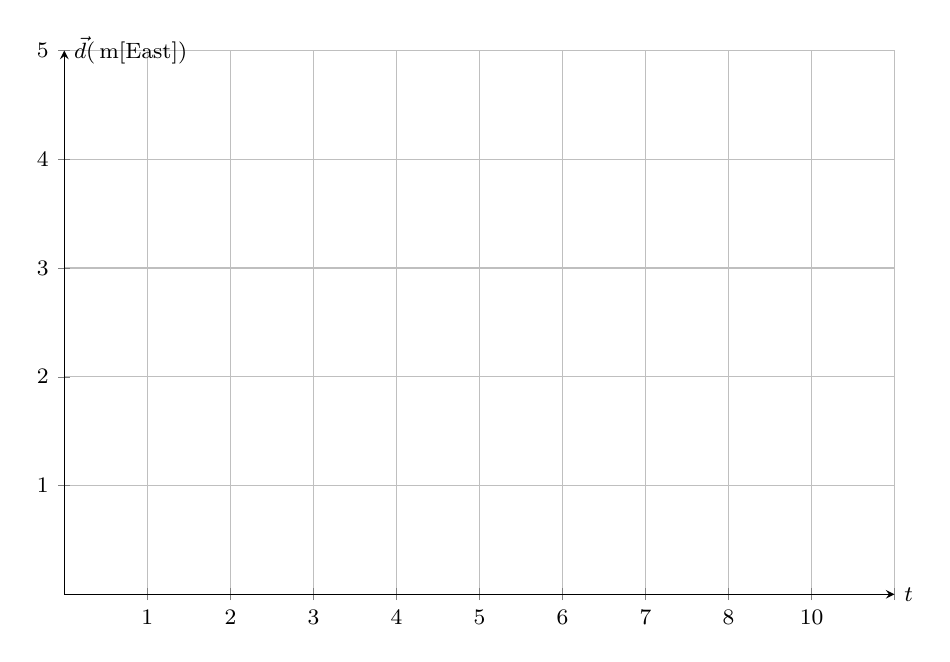
\begin{tikzpicture}
	\begin{axis}[
		my axis style,
		grid,
		yticklabels={1,2,1,2,3,4,5,6,7,8,9,10},	
		xticklabels={1,2,1,2,3,4,5,6,7,8,10},
		width=\textwidth,
		height=0.7\textwidth
	]

	\fill[
		black
	];
	
	\end{axis}
	\end{tikzpicture}
	\end{center}

\end{qstn}



\begin{qstn}[8]
Suppose that a wooden block slides down the ramp shown below at an average speed of $v_{av} = 10 \m / \s$. Suppose that it reaches point $M$ at $t = 4\s$.  Determine the height of the ramp (i.e Determine line segment $IA$).\\ (\textbf{Note: }We represent line segments in geometry from point $A$ to point $B$ as $AB$ or $BA$, this may be helpful in shortening your solution)
\begin{center}
	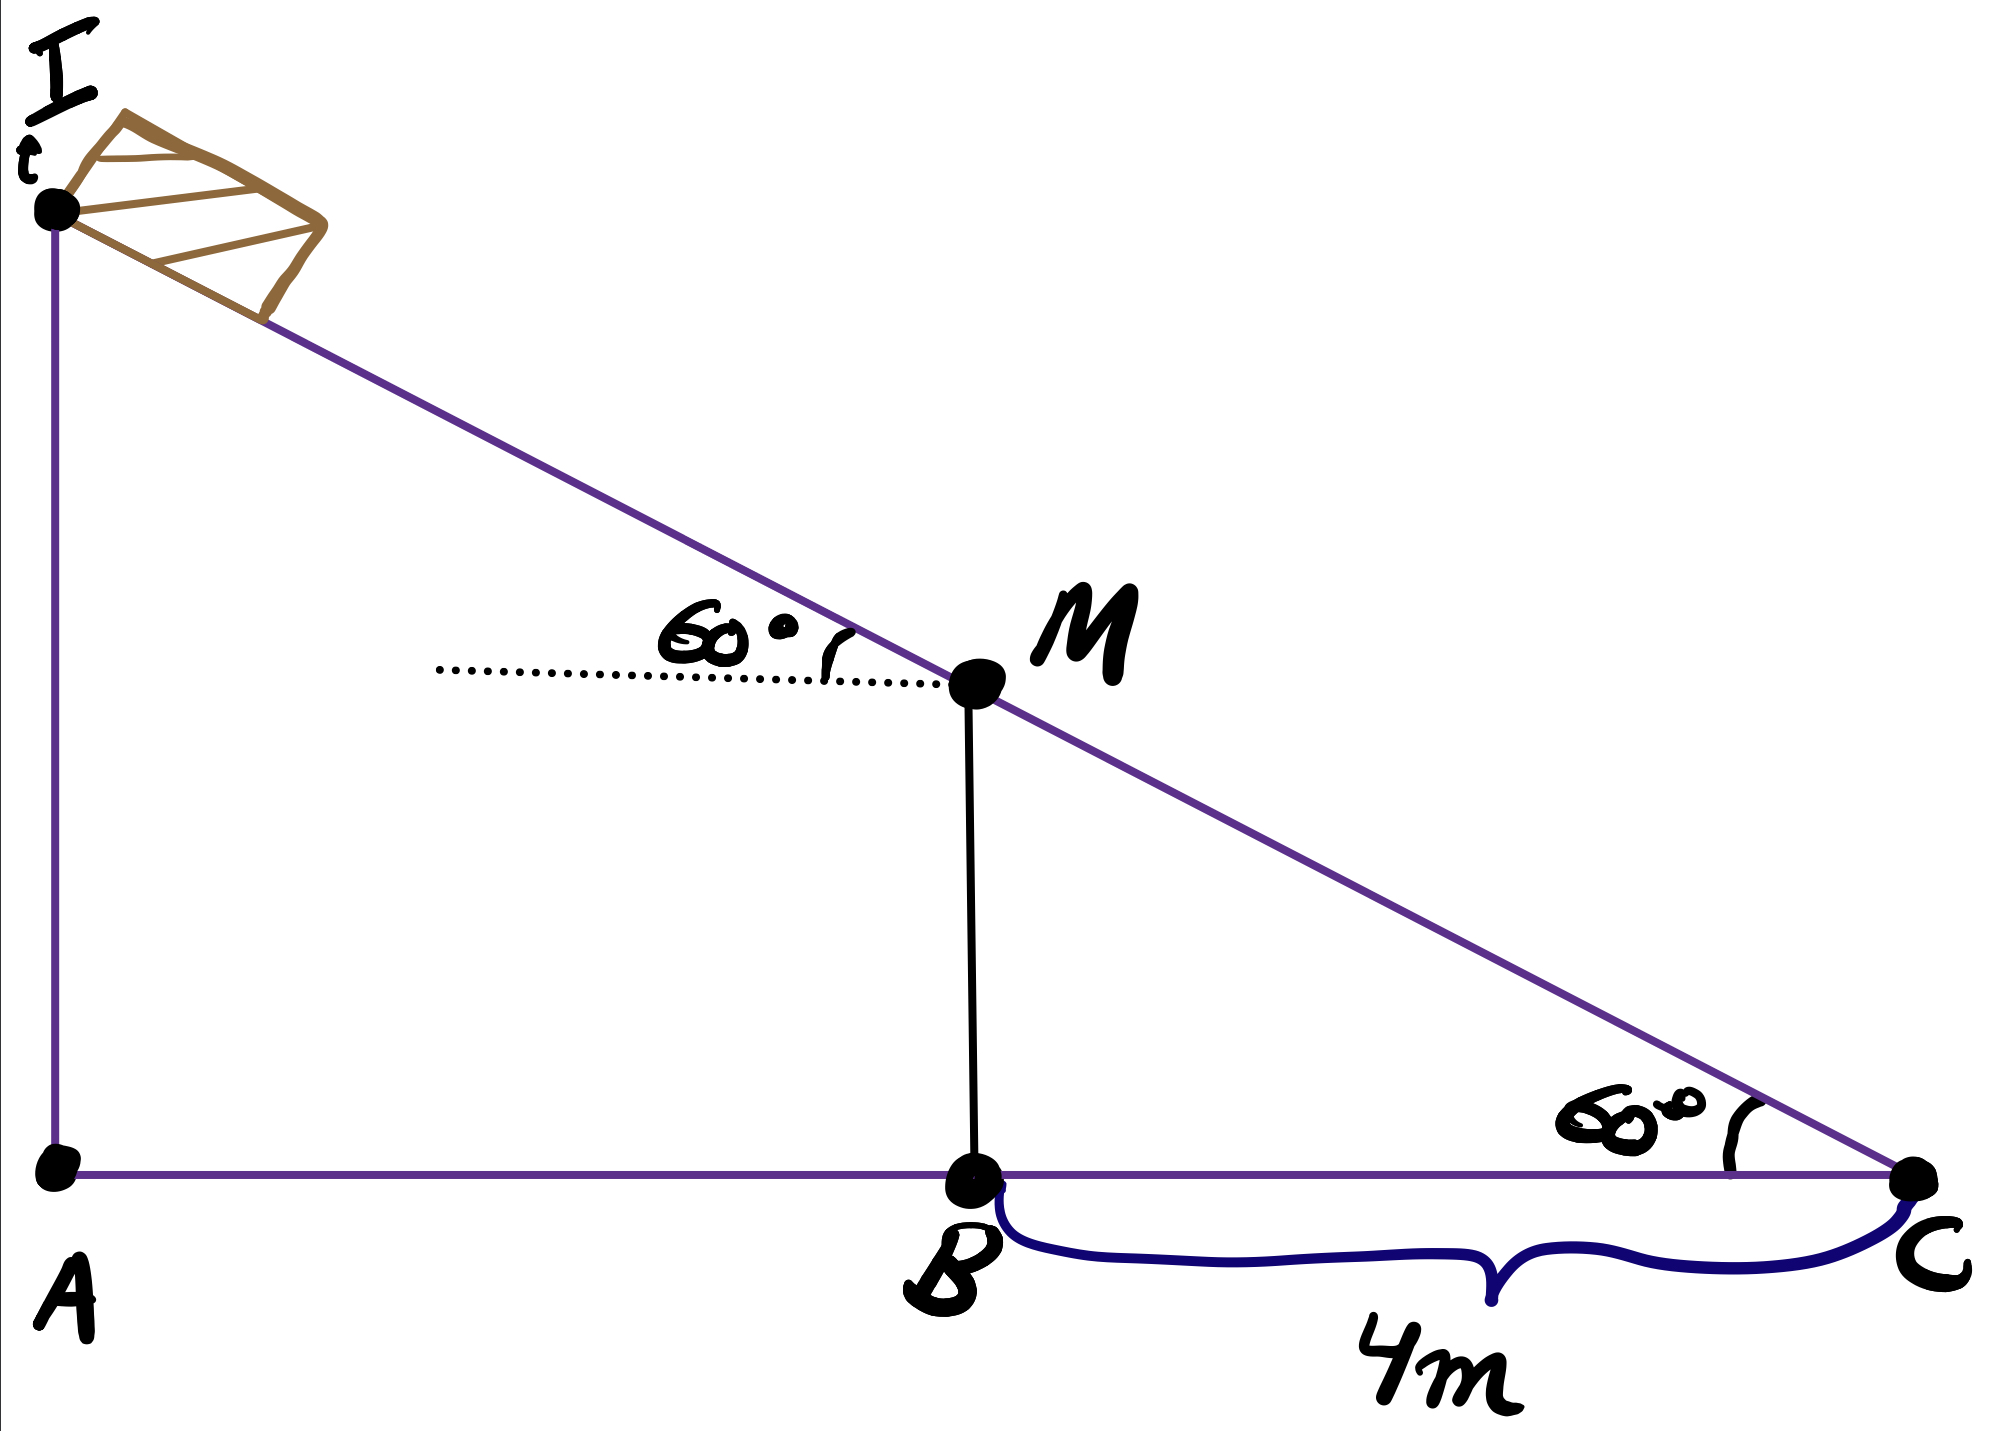
\includegraphics[width=13cm, height=10cm]{ramp.jpg}
\end{center}

\end{qstn}


\begin{qstn}[9]
Suppose that we have a straight line with three lights $A,B,C$. Suppose that we have the relative position vectors of these lights, $\vec d_{AB} = 56\m\tx{[East]}$, $\vec d_{CB} = 36\m\tx{[West]}$. Suppose that starting at light $A$, I traveled to the following sequence of lights $\{A,C,B,A,B,C\}$. If the entire journey took $\Delta t = 5\m$, compute my average velocity over the journey as well as my average speed. (In $\m / \s$) 

\end{qstn}


\begin{qstn}[10]
Suppose that I fire an arrow straight up into the air from a cliff at a position $\vec d_{CG} = 56\m$[North] relative to the ground. Suppose that a wooden box $14\m$ high is lying on the ground, and that the arrow lands directly on top of it. Compute the average velocity as well as the average speed of the arrow if the duration of the flight was $\Delta t = 45\s$. 
\end{qstn}

\begin{qstn}[11]
Suppose that I kick a soccer ball across a $150\m$ wide field and that by the end of its flight it lands in a ditch $24\m$ deep. What was the vertical displacement of the ball? What was the horizontal displacement of the ball? 

\end{qstn}

\begin{qstn}[12]
Suppose that a train coasting at an average speed of $250 \m / \s$ is headed for a mis-aligned track at a distance $2000\m$ ahead. A man on the train quickly grabs his scooter (which he had hidden away in his luggage) descends the train and attempts to switch the tracks alignment before the train reaches it. The scooter can ride at a maximum average speed of $300 \m / \s$. The train itself needs at least $3$ seconds in order to come to a complete stop. Can the man successfully switch the track in time? Prove that your answer is correct

\begin{soln}
\begin{proof}
	For this problem, we know that the the time the train needs is at least 3 seconds. Lets say that the time that the train takes to reach the mis-aligned track is t seconds. Since we need at least 3 seconds to come to a complete stop, the man on the scooter must reach the track in (t - 3) seconds at the latest.

	For ex : If the time it will take for the train to reach the track is t = 12 seconds, then the man has to reach the track at t = 9 seconds at the latest, anything after that is too late!
	
	Now we have the setup, all we need to do is compute the time that the man on the scooter will reach the track if he travels at his maximum speed and compare that to the time it takes for the train to reach the track.
	
	Time it takes for the train to reach the track : (2000) / 250 = 8 s
	
	Time it takes for the man on the scooter to reach the track 
	  = (2000) / 300 = 6.67
	
	We mentioned that the man on the scooter must reach the track at (t - 3) seconds at the latest, where t = time it takes for the train to reach the track. So (8 - 3) = 5 seconds is the latest time where he is allowed to reach the track, However the time where he reaches the track is 6.67 seconds, and this is beyond the latest time where he is allowed to reach the track. Therefore, the man cannot successfully switch the track in time. 

\end{proof}

\end{soln}

\end{qstn}

\end{document}

















